\documentclass[oneside,final,14pt]{extarticle}
\usepackage[utf8]{inputenc}
\usepackage[russian]{babel}
\usepackage{a4wide}
\usepackage{vmargin}
\usepackage{textcomp}
\usepackage{graphicx}
\newcommand*{\No}{\textnumero}
\setpapersize{A4}
\setmarginsrb{3cm}{2cm}{1cm}{2cm}{0pt}{0mm}{0pt}{13mm}
\usepackage{indentfirst}
\sloppy
\setcounter{page}{2}
\clubpenalty = 10000
\widowpenalty = 10000

\begin{document}

\thispagestyle{empty}

\begin{center}
\vspace{-3cm}


\includegraphics[width=0.5\textwidth]{msu.pdf}\\
{\scshape Московский государственный университет имени М.~В.~Ломоносова}\\
Факультет вычислительной математики и кибернетики\\
Кафедра алгоритмических языков

\vfill

{\LARGE Отчёт о выполнении задания практикума}

\vspace{1cm}

    {\Huge\bfseries <<Ассистент в бронировании>>}
\end{center}

\vspace{1cm}

\begin{flushright}
  \large
    \textit{Студент 325 группы}\\
  М.\,А.~Гулак\\
\end{flushright}

\vfill

\begin{center}
Москва, 2023
\end{center}

\newpage
\section{Постановка задачи}

Требуется реализовать программу, в диалоге с которой пользователь может
забронировать номер в гостинице. Для гостиницы известны вид номеров
и их количество, посуточная оплата, а также их текущая занятость на ближайшую неделю.
Вся эта информация о гостинице задается в текстовом файле и включает данные об уже
забронированных номерах гостиницы.

Исходный запрос пользователя на бронирование может быть определен частично
(например, не задан вид номера гостиницы), и в ходе диалога ему предлагаются возможные варианты бронирования и
уточняются все его детали (в случае ошибок ввода делаются подсказки). В конце диалога
выводится детальное описание произведенного бронирования.

Диалог может допускать возможность отмены или изменения бронирования. Также по
специальному запросу может быть выведена (для администрации гостиницы) вся
информация о забронированных на неделю номерах.

\subsection{Базовые требования}
    \begin{enumerate}
        \item Загрузка внутренного представления отеля из файла. 
        % \item Реализация внутреннего представления отеля, а также комнат.
        \item Выявление ошибок в файле.
        \item Обработка пользовательского запроса, в том числе ошибок в нём.
        \item Возможности отменить или изменить запрос.
        \item Отображение занятости отеля на неделю по специальному запросу.
    \end{enumerate}

\subsection{Идивидуальные части}
    \begin{enumerate}
        \item Обновление текстового файла после окончания работы в программе.
        \item Проверка существования файла с данными об отеле.
    \end{enumerate}
\section{Модули проекта}

Проект состоит из следующих модулей:
\begin{itemize}
    \item \texttt{DataTypes.hs}~--- объявление основных типов;
    \item \texttt{Constants.hs}~--- константы.
    \item \texttt{TypesHandle.hs}~--- реализация функций для работы с новыми типами данных;
    \item \texttt{Book.hs}~--- реализация функций для диалога с пользователем и логики самого диалога;
    \item \texttt{Main.hs}~--- модуль с главной функцией, с которой начинается работа.
\end{itemize}

В модуле \texttt{DataTypes.hs} описаны следующие типы:
\begin{itemize}
    \item \texttt{Day}~--- описывает день недели, соответственно, 
    содержит 7 значений;
    \item \texttt{RoomType}~--- описывает тип комнаты: одиночная или двойная;
    \item \texttt{Room}~--- структура для описания комнаты, имеющая поля:
    \begin{itemize}
        \item \texttt{roomId}~--- номер комнаты;
        \item \texttt{rommType}~--- тип комнаты;
        \item \texttt{roomPrice}~--- стоимость комнаты;
        \item \texttt{roomBookWeek}~--- занятость комнаты на неделю.
    \end{itemize}
    \item \texttt{Hotel}~--- структура для описания отеля, имеющая поля:
    \begin{itemize}   
        \item \texttt{hotelName}~--- название отеля;
        \item \texttt{hotelTypes}~--- типы комнат отеля;
        \item \texttt{hotelRoomAmount}~--- количество комнат;
        \item \texttt{hotelBusy}~--- занятость отеля на неделю.
    \end{itemize}
    \item \texttt{Request}~--- структура для описания запроса пользователя, имеющая поля:
    \begin{itemize}  
        \item \texttt{roomtype}~--- тип комнаты;
        \item \texttt{days}~--- список дней для бронирования.
    \end{itemize}
\end{itemize}

В модуле \texttt{Constants.hs} описаны следующие константы:
\begin{itemize}
    \item \texttt{week}~--- список дней недели;
    \item \texttt{weekS1}, \texttt{weekS2} и \texttt{weekS} ~--- списки 
    дней недели в виде строк в полном и сокращённом 
    виде соответственно, а также объединение этих списков;
    \item \texttt{typeS}~--- список типов комнаты в виде строк;
    \item \texttt{assocWeekSD}~--- ассоциативный список для перевода 
    дня недели из строки в соответствующий тип данных;
    \item \texttt{requestPrompts}~--- список подсказок при получении запроса;
    \item \texttt{help}~--- список для проверки правильности запроса.
\end{itemize}

В модуле \texttt{TypesHandle.hs} описаны следующие функции:
\begin{itemize}
    \item \texttt{transformFile}~--- перевод файла в виде строки в 
    список комнат и структуру \texttt{Hotel};
    \item \texttt{parseFile}~--- разбиение списка строк файла на имя отеля 
    и список комнат;
    \item \texttt{initializeHotel}~--- инициализация типа данных Hotel по его 
    имени и списку комнат;
    \item \texttt{initializeRooms}~--- инициализация типа данных Room по списку 
    строк;
    \item \texttt{weekBusy} и \texttt{weekBusyHelp}~--- создание списка занятости 
    отеля на неделю;
    \item \texttt{addToBusy}~--- обновление списка занятости;
    \item \texttt{stringToRoom}, \texttt{roomToString}~--- перевод строки, 
    соответствующей номеру отеля из файла, в тип данных \texttt{Room} 
    и обратно;
    \item \texttt{transformDaysToBool},\texttt{transformDaysFromBool}~--- 
    перевод списка дней недели из списка строк или дней в формате 
    \texttt{Day} в список True/False и обратно;
    \item \texttt{updateRoom}~--- обновление одной комнаты в соответствии 
    с запросом пользователя;
    \item \texttt{updateRooms}~--- обновление списка комнат;
    \item \texttt{updateHotel}~--- обновление отеля по одной комнате;
    \item \texttt{findRooms}~--- поиск списка комнат, подходящих под 
    запрос пользователя;
    \item \texttt{isRoomBusy}~--- проверка занятности комнаты;
    \item \texttt{showRoom}~--- преобразование комнаты в строку 
    для вывода на экран;
    \item \texttt{showRooms}~--- преобразование списка комнат в строку 
    для вывода на экран;
    \item \texttt{showBusy}, \texttt{showBusyHelp} и \texttt{showBusyDay}
    ~--- преобразование списка занятости отеля в строку для вывода на экран;
    \item \texttt{transform}~--- преобразование запроса из списка строк
    в список запросов;
    \item \texttt{transformDaysIntervalToBool} и \texttt{transformOneDay}
    ~--- преобразование интервала дней недели в список True/False. 
\end{itemize}

В модуле \texttt{Book.hs} описаны следующие функции:
\begin{itemize}
    \item \texttt{fullRequestHandle}~--- обработка запроса пользователя;
    \item \texttt{getInitialRequest}~--- получение начального запроса от пользователя
    (может быть как полным, так и неполным);
    \item \texttt{processReq}~--- уточнение запроса и поиск комнат по запросу;
    \item \texttt{getRequest}~--- получение уточнённого запроса от 
    пользователя;
    \item \texttt{book}~--- бронирование комнаты;
    \item \texttt{run}~--- основная функция обработки всех команд.
\end{itemize}

\section{Используемые библиотеки}

При реализации использовались следующие библиотеки:
\begin{itemize}
    \item \texttt{Data.Maybe}
    \item \texttt{Text.Read} 
\end{itemize}

\section{Сценарии работы с приложением}

Для начала работы необходимо запустить в интерпретаторе ghci файл 
\texttt{Main.hs}, а в нём~--- функцию \texttt{main}.
После запуска пользователю будет предложено ввести название файла, в котором 
хранится информация об отеле. После этого 

В случае ввода названия несуществующего файла будет выведено следующее сообщение:
\begin{center}
    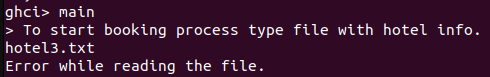
\includegraphics[width=0.75\textwidth]{picture03.png}
\end{center}

Если же файл существует, но в нём есть ошибка, не позволяющая инициализировать внутреннее 
представление, то будет выведено сообщение:
\begin{center}
    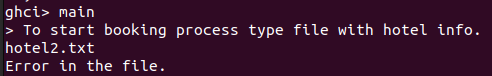
\includegraphics[width=0.75\textwidth]{picture02.png},
\end{center}
либо
\begin{center}
    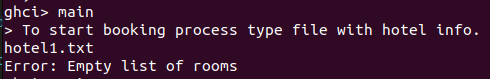
\includegraphics[width=0.75\textwidth]{picture01.png}
\end{center}

Если с файлом всё в порядке, то будет выведена информация об отеле
(его название), а также о доступных командах.
\begin{center}
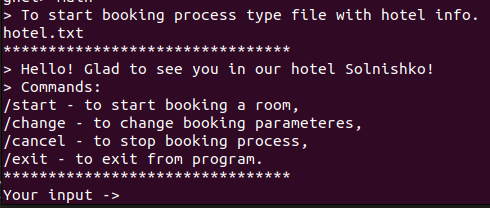
\includegraphics[width=0.75\textwidth]{picture1.png}
\end{center}

Далее для начала процедуры бронирования нужно ввести \texttt{/start}.
Пользователю будет предложено ввести запрос в виде "День заезда, день выезда, 
тип комнаты". Последний параметр необязателен на этом этапе, его можно не вводить.
\begin{center}
    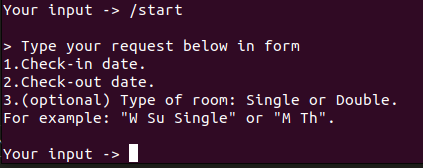
\includegraphics[width=0.75\textwidth]{picture2.png}
\end{center}
На этом этапе пользователь может отменить бронирование, либо ввести свой запрос.
После ввода запроса будут выведены все доступные варианты.
\begin{center}
    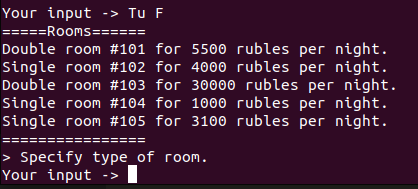
\includegraphics[width=0.75\textwidth]{picture3.png}
\end{center}

Если запрос был неполным, то после просмотра результатов нужно будет его дополнить 
необходимым типом комнаты.
\begin{center}
    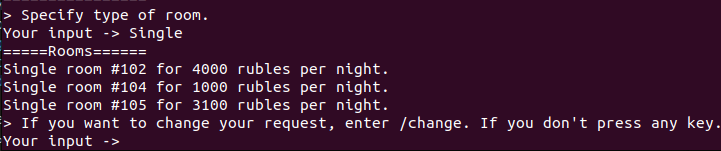
\includegraphics[width=\textwidth]{picture4.png}
\end{center}

После этого можно изменить запрос, введя команду \texttt{/change}, тогда просто процесс 
брони начнёться заново. Если нажать любую клавишу, то пользователю будет предложено выбрать 
номер комнаты, которую он хочет забронировать. После выбора комнаты будет показана ещё 
раз информация об этой комнате. На этом процесс бронирования заканчивается.
\begin{center}
    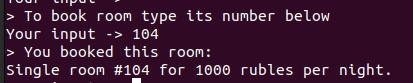
\includegraphics[width=0.75\textwidth]{picture5.png}
\end{center}

С помощью специальной команды \texttt{/admin} можно посмотреть всю занятость отеля на 
неделе.
\begin{center}
    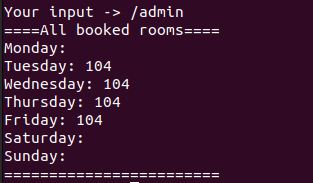
\includegraphics[width=0.75\textwidth]{picture6.png}
\end{center}

Как видно на скриншоте, здесь отобразился забронированный ранее номер 104.

Данные, которые вводит пользователь, проверяются на корректность и программа ожидает 
от пользователя подходящего ввода.
\begin{center}
    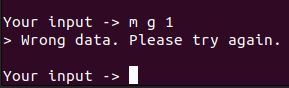
\includegraphics[width=0.75\textwidth]{picture71.png}
\end{center}
\end{document}
